	\hypertarget{resultados}{\section{Resultados}}
En esta sección se muestran las secciones transversales para elipsoides oblatos, empleados como una primera aproximación a la forma discoide cóncava de los eritrocitos. Dado que los eritrocitos en una muestra real no interactúan fuertemente entre ellos \footnote{El contraste en el índice de refracción entre los eritrocitos y el plasma sanguíneo es relativamente bajo (0.04 - 0.06) \cite{Blood}.} y que se encuentran orientados de forma aleatoria, se estudia la respuesta óptica promedio de una sola partícula, al considerar que una onda plana  ilumina a una colección de eritrocitos idénticos no interactuantes.  Por la aleatoridad de los elipsoides considerados, se emplea la respuesta promedio, que considera la excitación de un elipsoide a los largo de sus tres semiejes. De esta forma, las secciones transversales promedio de absorción y esparcimiento se expresan como \cite{Bohren}:
\begin{align*}
	\langle C_{abs}\rangle &= \frac{k}{3} \text{Im}\{\alpha^{(1)}+\alpha^{(2)}+\alpha^{(3)}\},\\
	\langle C_{sca}\rangle &= \frac{k^4}{3(6\pi)} \left(\alpha^{(1)}+\alpha^{(2)}+\alpha^{(3)}\right)^2.
\end{align*}

Para modelar la respuesta electromagnética del material de los elipsoides, se propone emplear el modelo de Drude. Este modelo describe el comportamiento plasmónico de materiales a energías bajas, es decir, aquella dominada por los electrones en la banda de conducción. Al considerar que una colección de electrones no interactuantes entre sí de un material se encuentran bajo la presencia de un campo eléctrico armónico con una frecuencia $\omega$, la expresión de la función dieléctrica dada por el modelo de Drude es \cite{Plasmonics}
\begin{equation} \epsilon(\omega) = 1 - \frac{\omega_p^2}{\omega^2 + i\gamma\omega}, 
\label{Drude}
\end{equation}
donde $\omega_p$ es la frecuencia de plasma y $\gamma$ es la constante fenomenológica de amortiguamiento, ambas características de cada material. A pesar de  que los eritrocitos no están compuestos por materiales dominados por un comportamiento plasmónico en el espectro visible, se emplea el modelo de Drude debido a su dependencia en la frecuencia, lo que permite, al seleccionar los parámetros $\omega_p$ y $\gamma$, un control sobre la respuesta óptica del sistema, resultando adecuado para estudiar la respuesta general y familiarizarse con el problema.\\

Para analizar la respuesta óptica en partículas elipsoidales dentro del régimen cuasiestático al compararlas con la respuesta de una esfera, se emplea inicialmente la función dieléctrica del aluminio dada por el modelo de Drude con los parámetros $\hbar\omega_p=13.142\text{ eV}$ y $\hbar\gamma=0.197\text{ eV}$ \cite{Aluminio}. Además, como la función dieléctrica del plasma, medio en el cual están inmersos los eritrocitos, es de alrededor de 1.81 en el espectro visible \cite{Blood}, en los cálculos siguientes, como primera aproximación, se considerará a las partículas inmersas en un medio acuoso con función dieléctrica $\epsilon_m$=1.77. En la Fig. \ref{Contribuciones} se muestran las $\langle C_{abs} \rangle$ (línea verde oscuro) y $\langle C_{sca} \rangle$(línea verde claro) de  un elipse con semiejes $a=1.5\text{ nm}$, $c=1\text{ nm}$ y las $\langle C_{abs} \rangle$ (línea roja punteada) y $\langle C_{sca} \rangle$(línea naranja punteada) de una esfera con $c=1.5\text{ nm}$. Todas las cantidades se muestran
como función de la energía $\hbar\omega$ (eje inferior) y la longitud de onda $\lambda$ (eje superior) de la onda electromagnética incidente. \\
\begin{figure}[h!]
	\sidesubfloat[]{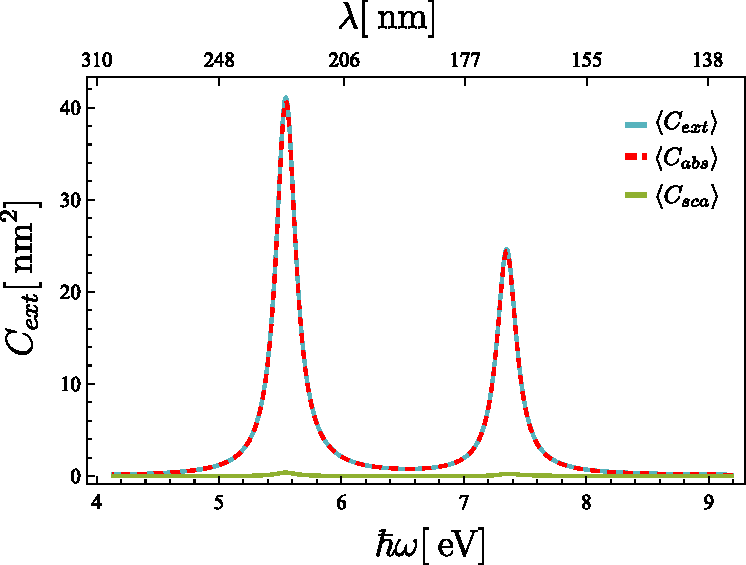
\includegraphics[width=.445\textwidth]{../../Figuras/AlContribuciones3.pdf} \label{Contribuciones}}\quad%
	\sidesubfloat[]{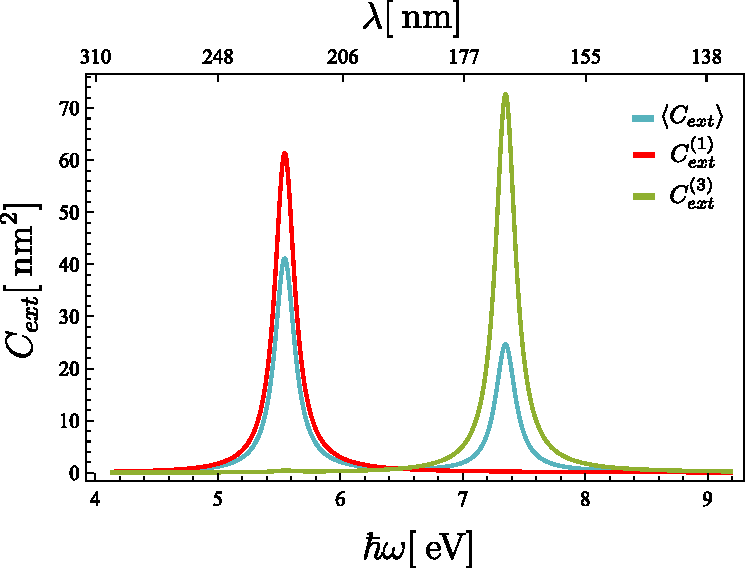
\includegraphics[width=.44\textwidth]{../../Figuras/CextAlbueno.pdf}\label{Cextpromedio}}%
	\caption{Secciones transversales como función de la energía $\hbar\omega$ (eje inferior) y de la longitud de onda $\lambda$ (eje superior) para una partícula elipsoidal oblata de aluminio caracterizada por su función dieléctrica dada por el modelo de Drude ($\hbar\omega_p=13.142\text{ eV}$, $\hbar\gamma=0.197\text{ eV}$), con semiejes $a=b=1.5\text{ nm}$, $c=1\text{ nm}$ e inmersa en un medio acuoso ($\epsilon_m=1.77$). \textbf{a)}~Sección transversal de absorción promedio $\langle C_{ext}\rangle$  del elipsoide (línea verde oscuro) y la esfera (línea roja punteada) y sección transversal de esparcimiento promedio $\langle C_{abs}\rangle$  del elipsoide (línea verde claro) y la esfera (línea naranja punteada) en escala logarítmica. \textbf{b)} Sección transversal de extinción promedio $\langle C_{ext}\rangle$ (línea azul), sección transversal de extinción al iluminar a la partícula con una onda polarizada en la dirección $\hat{e}_x$, $C_{ext}^{(1)}$  (línea roja)  y sección transversal de extinción al iluminar la partícula con una onda polarizada en la dirección $\hat{e}_z$ $C_{ext}^{(3)}$  (línea verde).} \label{fig:test}
\end{figure}

A partir de los resultados mostrados en la Fig. \ref{Contribuciones}, se observa que, en partículas dentro del régimen cuasiestático, la absorción domina sobre el esparcimiento en la contribución a la extinción. Esto se evidencia en la diferencia de magnitudes las curvas de absorción y esparcimiento de la esfera y la elipse, donde la absorción es aproximadamente tres órdenes de magnitud mayor que el esparcimiento, por lo que la curva de extinción es escencialmente la misma que la de absorción. Debido a esta marcada diferencia, los análisis posteriores se enfocan exclusivamente en las secciones transversales de extinción, ya que la contribución del esparcimiento es despreciable.\\

El análisis de las diferencias entre la $\langle C_{ext}\rangle$ y  las secciones transversales de extinción obtenidas al iluminar la partícula con una onda polarizada en una única dirección, se presenta en la Fig. \ref{Cextpromedio}. En esta figura se muestra la $\langle C_{ext}\rangle$ (línea azul), $C_{ext}^{(1)}$ (línea roja) y $C_{ext}^{(3)}$ (línea verde) de un elipsoide y la $\langle C_{ext}\rangle$ (línea gris punteada) de una esfera. Las cantidades se muestran en función de $\hbar\omega$ (eje inferior) y de $\lambda$ (eje superior) de la onda electromagnética incidente. Estos cálculos corresponden a un sistema con las mismas características que el de la Fig. \ref{Contribuciones}. Se observa que debido a la geometría, la 
$\langle C_{ext}\rangle$ del elipsoide presenta dos máximos, los cuales coinciden con las frecuencias de los máximos de $C_{ext}^{(1)}$ y $C_{ext}^{(3)}$ que se encuentran hacia el rojo y al azul, respectivamente, de la frecuencia de resonancia correspondiente a una partícula esférica. Esto muestra que las secciones transversales promedio son útiles para representar el efecto de iluminar una partícula elipsoidal con una onda electromagnética polarizada en la dirección de cualquiera de sus tres ejes principales, ya que lo que cambia es el valor nominal de los máximos en la sección transversal promedio, más no la localización espectral de estos. \\

Las siguientes figuras presentan los cálculos de las secciones tranversales de extinción promedio  $\langle C_{ext}\rangle$ considerando nanopartículas elipsoidales oblatas cuya función dieléctrica está caracterizada por el modelo de Drude para aluminio \cite{Aluminio} y por datos experimentales para plata \cite{Plata}, oro \cite{Plata}, bismuto \cite{Bismuto} y  óxido de magnesio \cite{MgO}.


\subsection*{Aluminio y plata}
En la Fig. \ref{aluminioplataAR} se muestran las $\langle C_{ext}\rangle$ en función de $\hbar\omega$ (eje inferior) y de  $\lambda$ (eje superior) de la onda electromagnética incidente en nanopartículas elipsoidales oblatas de aluminio (AlNPs) [Fig. \ref{aluminioAR}] y plata (AgNPs) [Fig.~\ref{plataAR}]. La función dieléctrica para el aluminio está dada por el modelo de Drude con parámetros $\hbar\omega_p=13.142\text{ eV}$, $\hbar\gamma=0.197\text{ eV}$, mientras que para la plata  está dada a partir de los datos experimentales reportados pr Johnson y Christy \cite{Plata}. Se realizan los cálculos para partículas elipsoidales con razón de aspecto AR=2 y con semiejes de tamaños desde 1 nm a 2.5 nm, en pasos de 0.5 nm; cada caso se identifica con el código de color mostrado en la gráfica. Además, se incluyen los cálculos para una partícula esférica con $a=2 \text{ nm}$ (línea gris punteada) y con razón de aspecto AR$=1$. Todas las partículas están  inmersas en un medio acuoso con $\epsilon_m=1.77$.\\

\begin{figure}[h!]
	\sidesubfloat[]{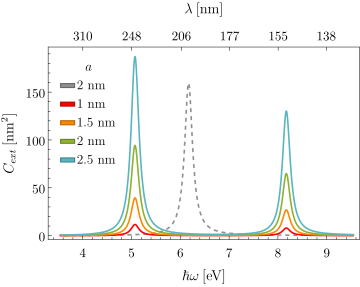
\includegraphics[width=.445\textwidth]{../../Figuras/AlAR} \label{aluminioAR}}\quad%
	\sidesubfloat[]{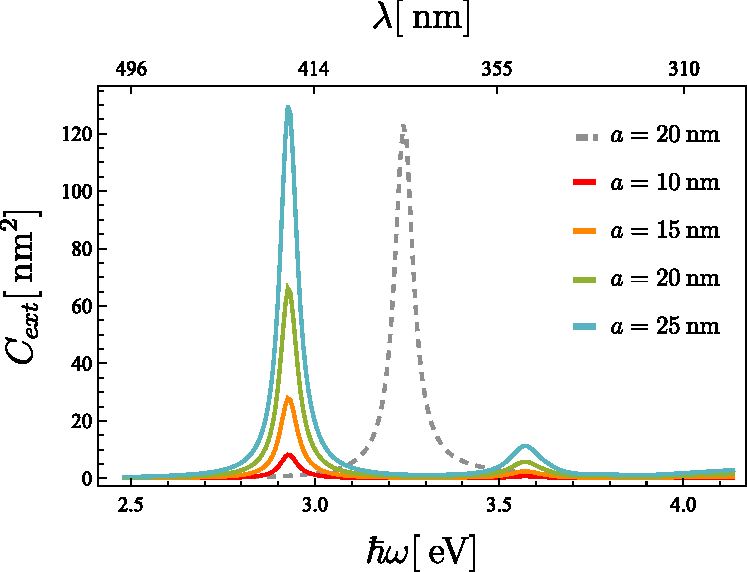
\includegraphics[width=.44\textwidth]{../../Figuras/AgAR}\label{plataAR}}%
	\caption{Secciones transversales de extinción promedio como función de la energía (eje inferior) y de la longitud de onda (eje superior) de la onda electromagnética incidente para una partícula elipsoidal oblata inmersa en un medio acuoso ($\epsilon_m=1.77$). Las partículas poseen AR=2, excepto en el caso de la línea gris punteada en el que AR=1 (partícula esférica). Además, están caracterizadas por su función dieléctrica dada por  \textbf{a)} el modelo de Drude para el aluminio con parámetros $\hbar\omega_p=13.142\text{ eV}$ y $\hbar\gamma=0.197\text{ eV}$) y \textbf{b)} datos experimentales correspondientes a la plata obtenidos de \cite{Plata}. }\label{aluminioplataAR}
\end{figure}
A partir de los resultados de la Fig. \ref{aluminioplataAR}, se observa que al aumentar el tamaño de la partícula mientras se mantiene constante AR, la localización espectral de las resonancias no cambia pero su valor nominal aumenta. Se identifican dos máximos locales en $\langle C_{ext}\rangle$,  los cuales corresponden a las frecuencias en las que $C_{ext}^{(1)}$ y $C_{ext}^{(3)}$ se maximizan. En ambos casos se observa que el corrimiento  de la resonancia no es simétrico respecto al de la esfera, para $C_{ext}^{(1)}$, las resonancias presentan un corrimiento hacia el rojo de $\Delta\lambda=$44 nm (1.11 eV) para las AlNPs y $\Delta\lambda=$51 nm (0.38 eV) para las AgNPs. Para $C_{ext}^{(3)}$, las resonancias presentan un corrimiento hacia el azul de $\Delta\lambda=$55 nm (2.33 eV) para AlNPs y $\Delta\lambda=$39 nm (0.36 eV) para las AgNPs. Es decir, este corrimiento depende del material.\\

El efecto de la variación de la razón de aspecto en la sección transversal de extinción promedio en AlNPs y AgNPs inmersas en un medio acuoso con $\epsilon_m=1.77$ se muestra en la Fig. \ref{aluminioplatac}. En esta figura, las partículas elipsoidales se consideran con AR entre 1.5 a 2.25, con incrementos 0.25 y con un semieje menor fijo de $c=1\text{ nm}$ y también se incluye $\langle C_{ext}\rangle$ para una partícula esférica con  $c=1\text{ nm}$ y con razón de aspecto AR$=1$.


\begin{figure}[h!]
	\sidesubfloat[]{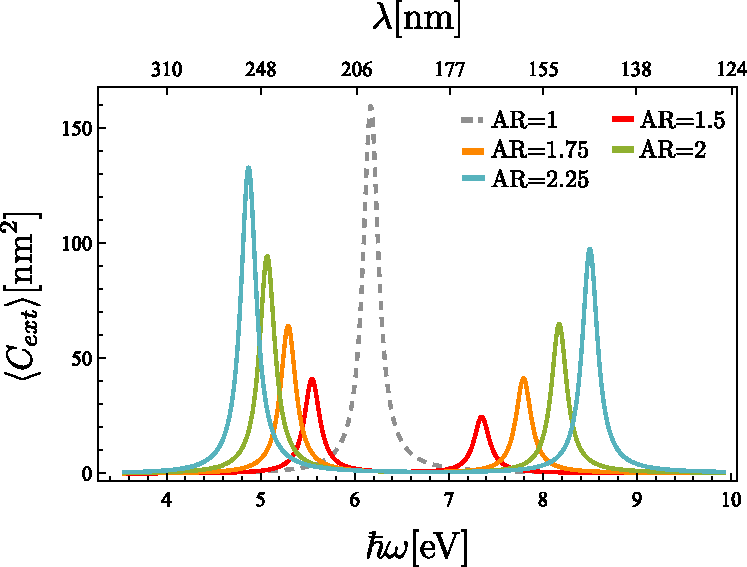
\includegraphics[width=.445\textwidth]{../../Figuras/Alc} \label{aluminioc}}\quad%
	\sidesubfloat[]{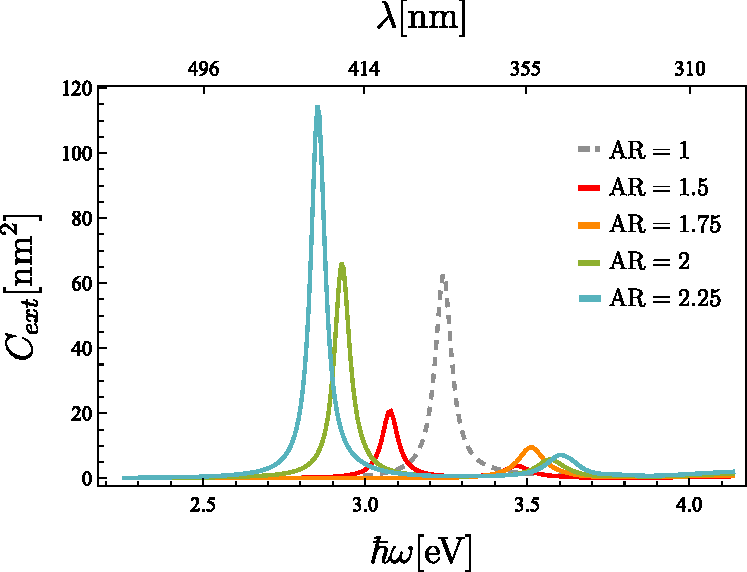
\includegraphics[width=.44\textwidth]{../../Figuras/Agc}\label{platac}}%
	\caption{Secciones transversales de extinción promedio como función de la energía (eje inferior) y de la longitud de onda (eje superior) de la onda electromagnética incidente para una partícula elipsoidal oblata inmersa en un medio acuoso ($\epsilon_m=1.77$). Las partículas  poseen un semieje menor de tamaño $c=1nm$ y presentan diferentes AR cuyo código de color se observa en la gráfica. Además, están inmersas en un medio acuoso ($\epsilon_m=1.77$) y están caracterizadas por su función dieléctrica dada por  \textbf{a)} el modelo de Drude para el aluminio ($\hbar\omega_p=13.142\text{ eV}$, $\hbar\gamma=0.197\text{ eV}$) y \textbf{b)} datos experimentales correspondientes a la plata obtenidos de \cite{Plata}.}\label{aluminioplatac}
\end{figure} 

 En las Figs. \ref{aluminioc}  y \ref{platac} se observa que conforme la relación de aspecto se aproxima a la unidad, hay un corrimiento de las frecuencias asociadas a las $\langle C_{ext}\rangle$ máximas hacia la frecuencia de resonancia asociada a una partícula esférica. Esta frecuencia de resonancia corresponde a $\lambda=201\text{ nm}$ (6.17 eV) para el aluminio y $\lambda=383\text{ nm}$ (3.24 eV) para la plata. Además, tanto en el aluminio como en la plata, se observa que al aumentar la relación de aspecto y la longitud del eje mayor, el valor nominal de  $\langle C_{ext}\rangle$ también aumenta. Esto se debe a que hay una mayor cantidad de material y por tanto más electrones, por lo que los efectos de absorción y esparcimiento aumentan, lo que, en consecuencia, aumenta la extinción.



\subsection*{Oro y bismuto}
De forma análoga al análisis en la variación de los parámetros geométricos de las AlNPs y AgNPs, se muestra en la Fig. \ref{oro} la respuesta óptica variando estos parámetros (semieje mayor y razón de aspecto) considerando ahora una función dieléctrica de materiales reales donde se observan contribuciones no descritas por el modelo de Drude. \footnote{Estas contribuciones provienen de electrones ligados \cite{Plasmonics}.} En particular, en la Fig. \ref{oroAR} se grafica $\langle C_{ext}\rangle$ como función de $\hbar\omega$ (eje inferior) y de $\lambda$ (eje superior) para nanopartículas elipsoidales oblatas de oro (AuNPs) de distintos tamaños que conservan la razón de aspecto de AR=2. Para complementar el análisis, se muestra debajo de esta gráfica la función dieléctrica del oro donde los puntos representan datos experimentales \cite{Plata} y las líneas continuas corresponden a la interpolación empleada para este conjunto de datos. En la Fig. \ref{oroAR} se consideran partículas con relación de aspecto AR$=2$ con radios desde 1  nm a 2.5 nm, con incrementos de 0.5 nm; cada caso se identifica con el código de color mostrado en la gráfica respectiva. También se considera una partícula con relación de aspecto AR$=1$ y semiejes $a=2$ nm (línea gris punteada), que representa a una partícula esférica. Por otro lado, en la Fig. \ref{oroc} se consideraron partículas con relación de aspecto variable AR=1.5 (línea roja), AR=1.75 (línea naranja), AR=2 (línea verde) y AR=2.25 (línea azul) que presentan valores en su semieje menor $c=1\text{ nm}$. Asimismo, se considera una partícula esférica con semieje mejor $c=1\text{ nm}$ y con relación de aspecto AR$=1$ (línea gris).
\begin{figure}[H]
	\sidesubfloat[]{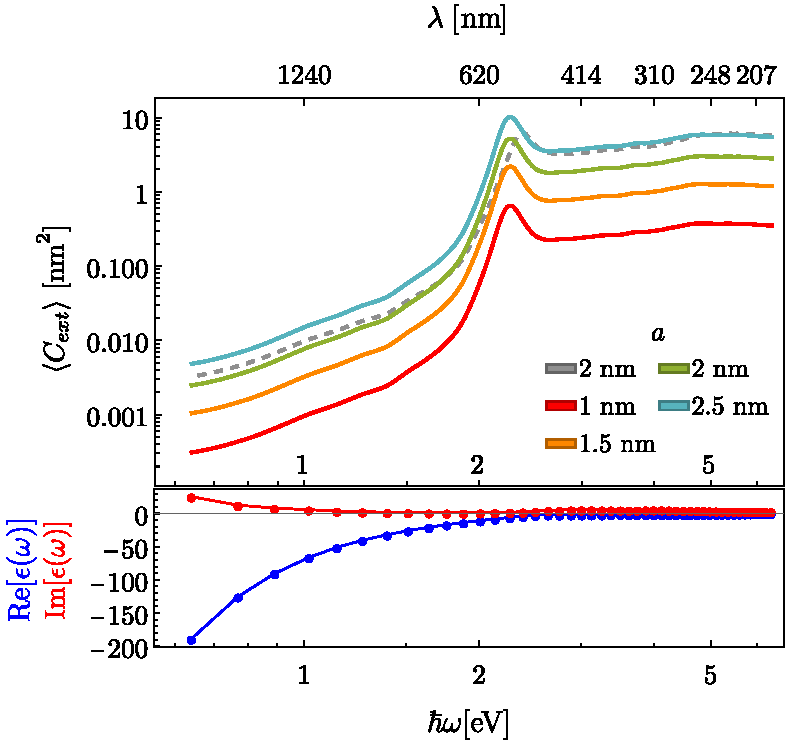
\includegraphics[width=.445\textwidth]{../../Figuras/Au2.pdf} \label{oroAR}}\quad%
	\sidesubfloat[]{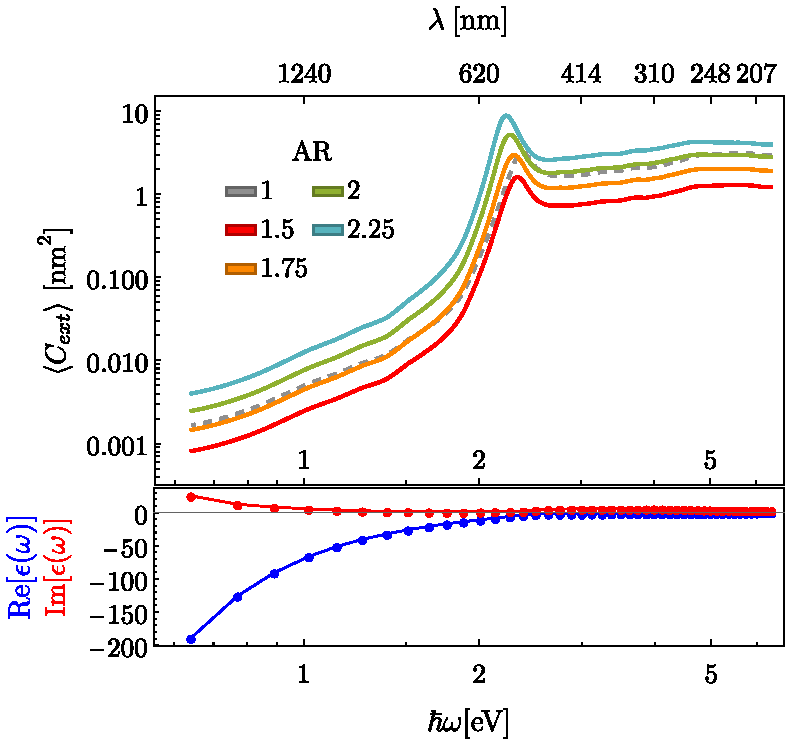
\includegraphics[width=.44\textwidth]{../../Figuras/Au.pdf}\label{oroc}}%
	\caption{Secciones transversales de extinción promedio como función de la energía (eje inferior) y de la longitud de onda (eje superior) para una partícula elipsoidal oblata de oro inmersa en un medio acuoso con $\epsilon_m=1.77$, y cuyo índice de refracción complejo fue obtenido a partir de datos experimentales de \cite{Plata}. Debajo de las gráficas se muestra la función dieléctrica del oro obtenida a partir de \cite{Plata} (parte real en azul, parte imaginaria en rojo). La línea recta que une los puntos experimentales fue obtenida mediante una interpolación. \textbf{a)} AuNPs con AR=2, excepto en el caso de una esfera (línea gris punteada) donde AR=1. \textbf{b)} AuNPs con semieje menor $c=1$ nm.}\label{oro}
\end{figure}

En contraste con el aluminio y la plata, para el oro se observa solo una excitación plasmónica en $\lambda=$ 522 nm (2.38 eV). Esta excitación presenta un corrimiento hacia el rojo de la de la esfera en $\lambda=$ 547 nm (2.27 eV) y se esperaría que existiera otra con un corrimiento hacia el azul, más no hay una excitación a frecuencias mayores como sí se observó en el análisis de la Fig. \ref{aluminioplataAR}. Esto se atribuye a la fuerte absorción del oro a energías altas, lo que suprime resonancias atribuidas a contribuciones no descritas por el modelos de Drude en los datos experimentales.\footnote{En particular de contribuciones dieléctricas descritas por el modelo de Lorentz \cite{Plasmonics}.} Por otro lado, se observa que para AR=2.25, la excitación se encuentra en $\lambda=$ 556 nm (2.23~eV), mientras que para AR=1.5, el caso calculado más cercano al de una esfera, la excitación se encuentra en $\lambda=$~522~nm (2.33~eV), es decir, la AR reproduce el caso de una esfera en su respuesta espectral cuando tiende a la unidad, resultado que sigue las tendencias observadas en las AlNPs y AgNPs.\\

En los casos anteriores se analizó el aluminio, cuya respuesta óptica es bien descrita por el modelo de Drude, así como metales nobles como la plata y el oro. Ahora, con el objetivo de aproximarse a las propiedades ópticas de los eritrocitos, en la Fig. \ref{bismuto} se presentan las secciones transversales de extinción promedio en función de la energía (eje inferior) y la longitud de onda (eje superior) para nanopartículas elipsoidales oblatas de bismuto (BiNPs). Este material, al ser un semimetal, exhibe en ciertas regiones espectrales un comportamiento más similar al de los eritrocitos que los materiales previamente estudiados. Como complemento, debajo de las gráficas se muestra la función dieléctrica del bismuto obtenida de datos experimentales reportados por Hagemann et al. \cite{Bismuto}. En la Fig. \ref{bismutoAR} se consideraron partículas con  AR$=2$  y en la Fig. \ref{bismutoc} se consideraron partículas con relación de aspecto variable desde 1.5 hasta 2.25, con incrementos de 0.25. 

\begin{figure}[H]
	\sidesubfloat[]{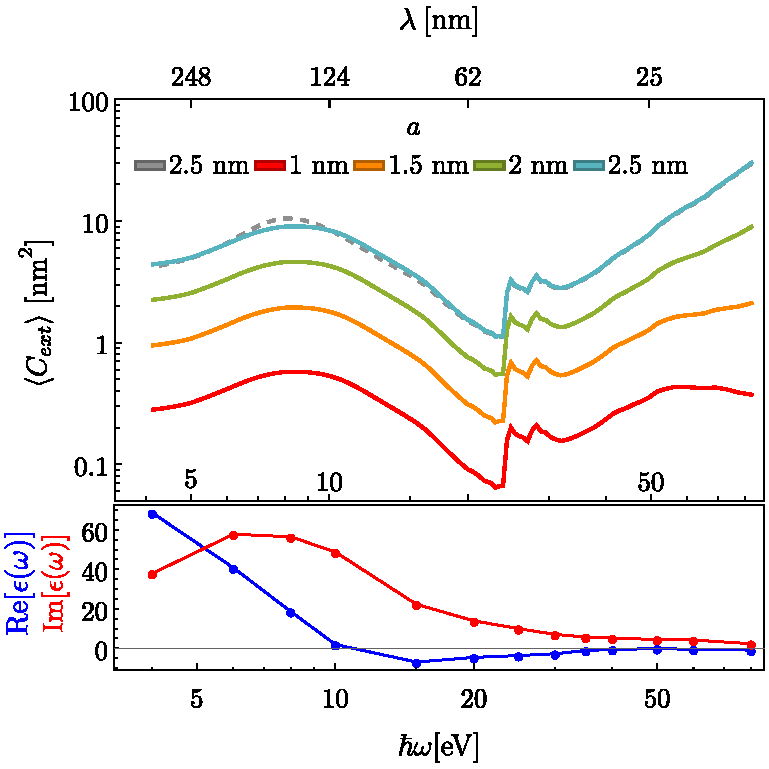
\includegraphics[width=.445\textwidth]{../../Figuras/Bi2} \label{bismutoAR}}\quad%
	\sidesubfloat[]{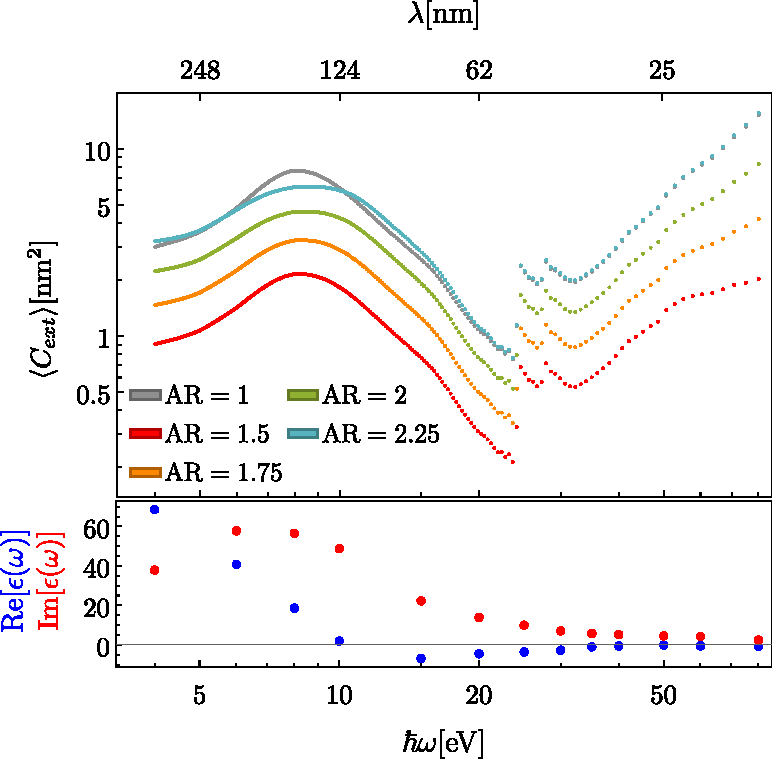
\includegraphics[width=.44\textwidth]{../../Figuras/Bi}\label{bismutoc}}%
	\caption{Secciones transversales de extinción promedio  como función de la energía (eje inferior) y de la longitud de onda (eje superior) para una partícula elipsoidal oblata de bismuto inmersa en un medio acuoso con $\epsilon_m=1.77$, y cuyo índice de refracción complejo fue obtenido a partir de datos experimentales de \cite{Bismuto}. Debajo de las gráficas se muestra la función dieléctrica del oro obtenida a partir de \cite{Plata} (parte real en azul, parte imaginaria en rojo). La línea recta que une los puntos experimentales fue obtenida mediante una interpolación. \textbf{a)} BiNPs con AR=2, excepto en el caso de una esfera (línea gris punteada) donde AR=1. \textbf{b)} BiNPs con semieje menor $c=1$ nm.}\label{bismuto}
\end{figure}

En ambas figuras se observan frecuencias de resonancia alrededor de $\lambda=147$ nm (8.44 eV), que se encuentran hacia el azul de la frecuencia de resonancia en $\lambda=154$ nm (8.03 eV) correspondiente a una nanopartícula esférica y de manera similar al caso del oro, se esperaría que existiera otra resonancia hacia el rojo de la de la esfera. También se observa un aumento de la $\langle C_{ext}\rangle$ a partir de $\lambda=50$ nm  que se atribuye a contribuciones no descritas por el modelo de Drude en los datos experimentales. Como en los casos anteriores, se observa que al aproximar AR a la unidad, se recupera la frecuencia de resonancia correspondiente a una nanopartícula esférica. Además, las excitaciones plasmónicas están menos definidas que en el caso de los materiales plasmónicos. Esto es más evidente al comparar la Anchura a media altura (FWHM por sus siglas en inglés) pues, en el caso del bismuto se observa un FWHM = 8.85 nm (0.18 eV), mientras que en el aluminio FHWM = 68.54 nm (3.64 eV). Esto se explica debido a la fuerte absorción del bismuto en el rango de frecuencias estudiado.





\subsection*{Óxido de magnesio}
Finalmente, las $\langle C_{ext}\rangle$ para un material dieléctrico: el óxido de magnesio (MgO) se muestran en la Fig. \ref{mgo}, en las que se emplearon los datos experimentales reportados por Stephens y Malitson \cite{MgO}. En esta gráfica se realiza la variación de la AR y el semieje mayor en nanopartículas elipsoidales oblatas de óxido de magnesio (MgONPs). Las $\langle C_{ext}\rangle$ se grafican en función de la energía (eje inferior) y de la longitud de onda (eje superior). De la misma forma que con los materiales anteriores, se consideraron partículas con relación de aspecto AR$=2$ con radios desde 1  nm a 2.5 nm, con incrementos de 0.5 nm, con su respectivo código de color indicado en la gráfica [Fig. \ref{mgoAR}] y en la Fig. \ref{mgoc} se consideraron partículas con AR variable. 

\begin{figure}[H]
	\sidesubfloat[]{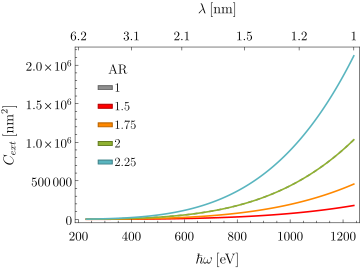
\includegraphics[width=.445\textwidth]{../../Figuras/MgOc} \label{mgoc}}\quad%
	\sidesubfloat[]{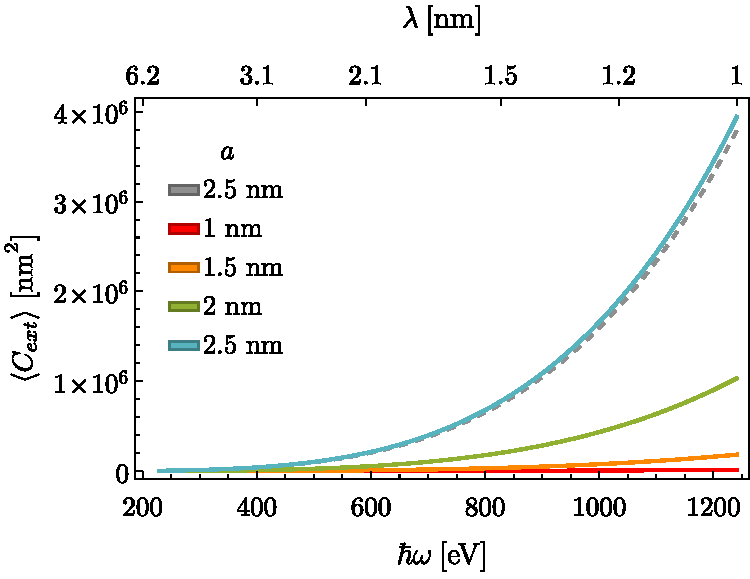
\includegraphics[width=.44\textwidth]{../../Figuras/MgOAR}\label{mgoAR}}%
	\caption{Secciones transversales de extinción promedio como función de la energía (eje inferior) y de la longitud de onda (eje superior) para una partícula elipsoidal oblata de óxido de magnesio inmersa en un medio acuoso ($\epsilon_m=1.77$). \textbf{a)} MgONPs con AR=2, excepto en el caso de una esfera (línea gris punteada) donde AR=1. \textbf{b)}  MgONPs con semieje menor $c=1$ nm.}\label{mgo}
\end{figure}

En ambos casos se observa que la $\langle C_{ext}\rangle$ tiene un comportamiento creciente y no se observan resonancias plasmónicas debido a la naturaleza dieléctrica del óxido de magnesio. Esto también se atribuye a que en el rango de energías analizado existen procesos de absorción no descritos por el modelo de Drude.








